%TEX root = ./overwiew.tex

\documentclass{standalone}

\usepackage{tikz}
\usepackage{smartdiagram}

\begin{document}

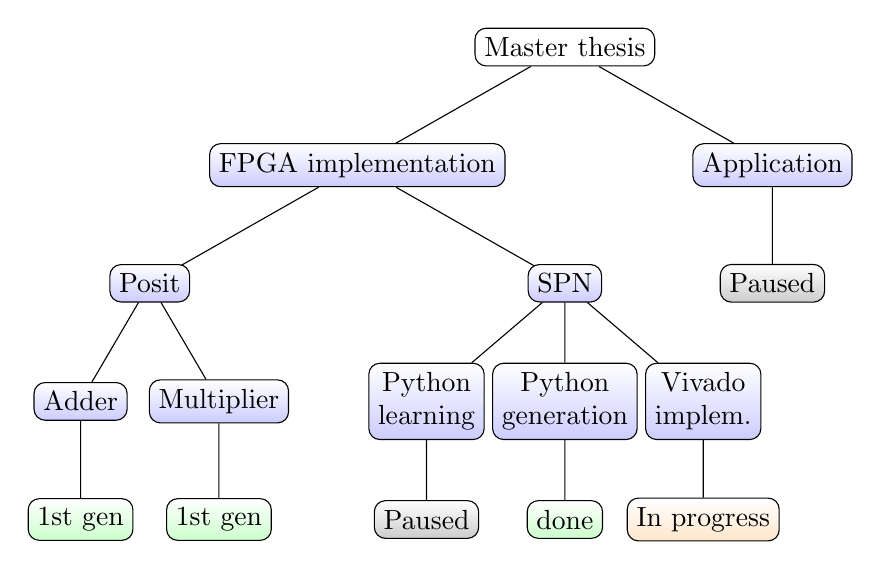
\begin{tikzpicture}[sibling distance=15em,
  	every node/.style = {shape=rectangle, rounded corners,
    draw, align=center},
    % top color=white, bottom color=blue!20}
    action/.style={top color=white, bottom color=blue!20},
    leaf_done/.style={top color=white, bottom color=green!20},
    leaf_todo/.style={top color=white, bottom color=orange!20},
    leaf_pause/.style={top color=white, bottom color=black!20},
    leaf_toimprove/.style={top color=white, bottom color=yellow!20},
    ]

    \node {Master thesis}
    child{ [sibling distance=15em] node [action] {FPGA implementation}
    	child{ [sibling distance=5em] node [action] {Posit}
    		child{ node [action] {Adder}
    			child{ node [leaf_done] {1st gen}}}
    		child{ node [action] {Multiplier}
    			child{ node [leaf_done] {1st gen}}}}
    	child{ [sibling distance=5em] node [action] {SPN}
    		child{ node [action] {Python\\learning}
    			child{ node [leaf_pause] {Paused}}}
    		child{ node [action] {Python\\generation}
    			child{ node [leaf_done] {done}}}
    		child{ node [action] {Vivado\\implem.}
    			child{ node [leaf_todo] {In progress}}}}}
    child{ node [action] {Application}
    	child{ node [leaf_pause] {Paused}}};

\end{tikzpicture}

\end{document}

